\section{A visualisation of the frame distribution with t-SNE}
\label{tsne}

In the previous sections I have extensively studied the case of the localisation within a journey, answering the question ``where am I along the path?'' that was introduced in Chapter \ref{ch:chapter2}. In a visual path retrieval system divided in different journeys inside a building, to be able to answer the question ``in which path am I on?'' with precision would give this system the necessary prior information to provide a better location and also suggest path planning, which would be specially relevant in an assistive context as we will see in Chapter \ref{ch:chapter6}. Although the journey selection was beyond the scope of this thesis, it was informative to study the behaviour of a state-of-the-art dimensionality reduction technique in a rather challenging scenario of having such highly dimensional data (the BOVW-encoded vectors have 4,000 elements). Therefore I chose t-SNE as a technique for visualising in two or three dimensions the high dimensional descriptor space of the RSM dataset.

t-distributed stochastic neighbour embedding (t-SNE) is a machine learning algorithm for dimensionality reduction developed by Laurens van der Maaten and Geoffrey Hinton \cite{maaten2009learning}. It is a non-linear dimensionality reduction technique that is particularly well suited for embedding high-dimensional data into a space of two or three dimensions, which can then be visualised in a scatter plot. Specifically, it models each high-dimensional object by a two- or three-dimensional point in such a way that similar objects are modelled by nearby points and dissimilar objects are modelled by distant points.

In other words, t-SNE is a dimensionality reduction technique that aims to preserve the local structure of the data. For this reason I wanted to compute the visual path descriptions of the RSM dataset and build the foundations for future work on journey/corridor selection.

\begin{figure}
\centering
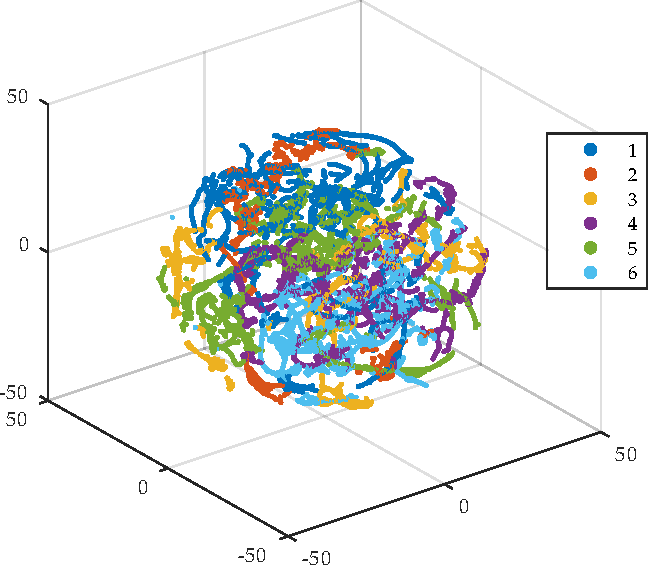
\includegraphics[width=\textwidth]{gfx/Chapter04/tsne_dsift_3d.pdf}
\caption{Distribution of the BOVW data of the RSM dataset in a reduced 3D space when visualised with t-SNE. Colours refer to different corridors in the dataset. Note that there is some evidence of the locally connected paths in the visual-words space.}
\label{fig:tsne3d}
\end{figure}

In Figure \ref{fig:tsne3d} we can see the 4,000-dimension visual word reduced to three dimensions and in Figure \ref{fig:tsne2d} we can see the two-dimensional embedding. The embeddings were generated using more than 50,000 randomly selected examples from all the corridors. Following the method described in Section~\ref{sec:quant_and_encod}, I selected for this particular example dense-SIFT descriptors encoded with hard assignment (HA), using $k$-means to create the visual word examples.

As we can see from the images, the difficulty of generating two or three-dimensional embeddings of such a high dimensional and complex dataset is notable. However, there are patterns showing how examples from the same corridors can display a sequential relationship within the embeddings.


\begin{figure}
\centering
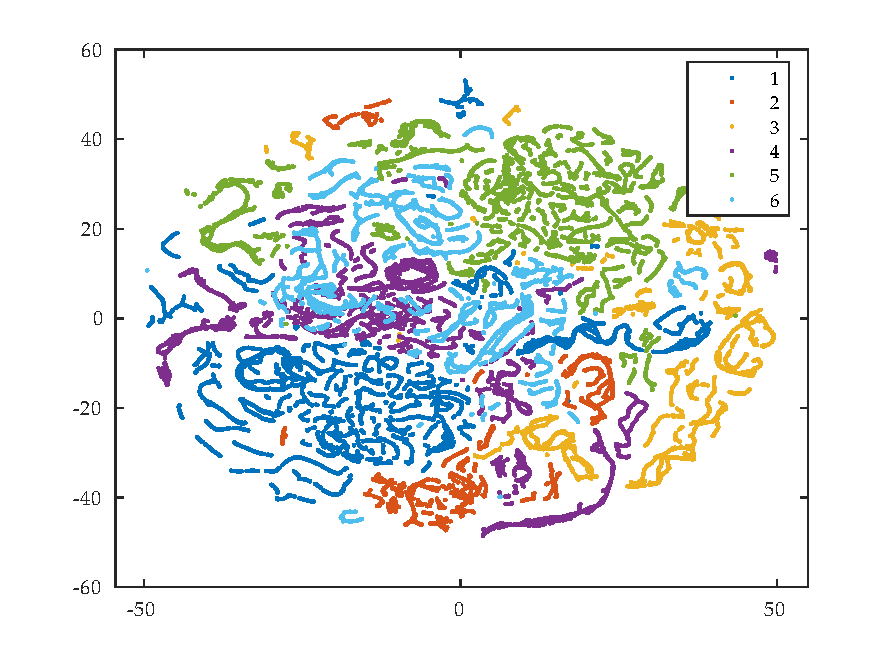
\includegraphics[width=\textwidth]{gfx/Chapter04/tsne_dsift_2d.pdf}
\caption{Distribution of the BOW data of the RSM dataset in a reduced 2D space when visualised with t-SNE. It is easy to identify some sets of points that form locally one-dimensional structures. Though they are not always contiguous for one corridor, the concept of visual paths appears at least partially justified.}
\label{fig:tsne2d}
\end{figure}

The present thesis gives an emphasis on understanding \textit{visual path} data from a journey perspective, from a crowdsourced collection of journeys in particular. However, although of limited practical use within journey localisation, this visualisation is the first step in understanding the structure of the data from a ``building'' perspective.

It is therefore subject of future work the use of these visualisations to understand the important features of visual paths datasets such as the presence of global clusters that reveal remarkable distinctiveness between journeys or give insight on how to optimise the retrieval based on between-journey differences.

